\chapter{Evaluation and Analysis}

In the first part of this section we briefly depict the nature of the data set used for evaluation of the models and discuss some specifics of the implementation. In the next part we present the results of our analysis.

\section{Data Set}

For the analysis we used data from the online system for practicing geography\footnote{\url{http://www.slepemapy.cz}}~\cite{Papousek2014}. The data set contains more than 10~million answers from thousands of unique users~\cite{Papousek2015}. The data were filtered to contain only students with at least 50 answers and usually divided into 5 data sets, each containing at least 30 thousand answers. The answers of students who registered before the oldest question in the data set was answered were removed since it could temper with the results (considering we are interested primarily in models based on timing information).

The used data set contains genuinely very different students with distinct prior knowledge, some students are still in school and practice geography in classes, other students already finished school and want to revive their forgotten knowledge (this is further analyzed in chapter~\ref{further-analysis}). There are also tremendous differences between continents, regions and types of places, all of which vary in the easiness of learning, some are harder to retain and are forgotten faster.

\section{Toolchain}

The models were implemented in Python programming language. Experiments were performed in the Jupyter Notebook interactive environment\footnote{Jupyter Notebook is an open sourced web application for interactive computing, see~\url{https://jupyter.org/}}. Here is a list of the used libraries and modules:

\begin{itemize}
  \item SciPy, NumPy, Pandas
  \item Matplotlib, Seaborn
  \item Scikit-Learn
  \item NetworkX
\end{itemize}

\section{Response Time}

The response time of student to a question indicates how much well the item is learned. If the student answered quickly, almost automatically, it is very likely they either know the place very well or don't at all, depending on the correctness of their answer. On the other hand when the response is longer, the student is probably familiar with the item and might even recall the correct answer.

The Figure~\ref{fig-response-time} demonstrates the relationship between students' response time and the probability of recall. If the student's answer was suspiciously fast (response time is lower than 800 milliseconds), it usually means they are guessing. If the response time is between 1500 and 2000 milliseconds, it may indicate the student knows the correct answer.

Note that some places are larger on the map then other, i.e. a question requiring the student to select Russia on the map has generally lower response time than a question requiring to select Andorra.

\begin{figure}[htbp]
  \centering
  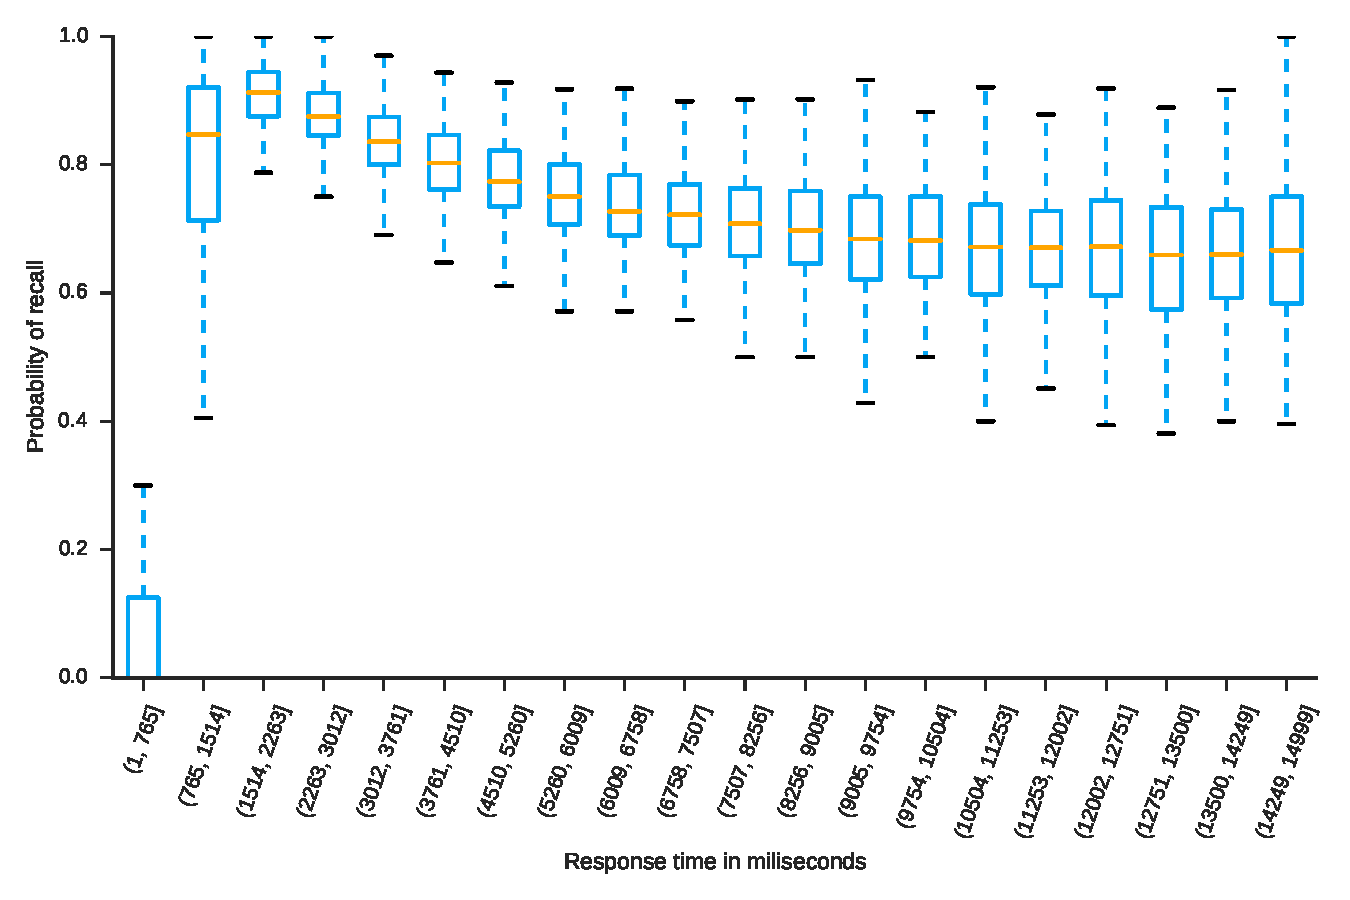
\includegraphics[width=\textwidth]{img/response-time}
  \caption{Relation between students' response time and probability of recall. Each box represents probabilities from all countries that belong in the relevant interval of response times.}
  \label{fig-response-time}
\end{figure}

TODO: describe the extended model here, evaluate and analyze.

\section{Memory Decay}

In this chapter we evaluate and analyze several models with the focus on memory decay and forgetting. Since we use abbreviations for the models, here is a list of all evaluated models as they occur in our experiments:

\begin{itemize}
  \item \textbf{PFA} -- this is the original performance factor analysis which we described in chapter~\ref{pfa}. Our implementation, however doesn't consider multiple knowledge components as there is only one.
  \item \textbf{PFA/E} -- a version of the original PFA model with some aspects of Elo model we depicted in chapter~\ref{pfae}.
  \item \textbf{PFA/E/T} -- an extended version of the PFA/E model which adapts the idea of a time effect function. We presented the model in chapter~\ref{pfaet}. In our analysis we examined several time effect functions.
  \item \textbf{PFA/G} -- another version of the original PFA model with a decay factor, the characteristics of the model were outlined in chapter~\ref{pfag}. The implementation doesn't consider multiple knowledge components.
  \item \textbf{PFA/G/T} -- our version of the PFA/G model which uses a time effect function instead of a decay factor. The differences were stated in chapter~\ref{pfagt}.
\end{itemize}

Note that for the estimation of prior knowledge we sometime use the Elo model briefly described in chapter~\ref{elo}. In any case, we always explicitly mention when the dedicated prior knowledge estimator is used.

\subsection{Parameters}
\label{parameters}

Standard PFA model has 3 parameters, the initial difficulty of an item $\beta$, weight of each success $\gamma$ and failure $\delta$. In cases where we use Elo model for prior knowledge estimation, we can replace the parameter $\beta$ with $\theta_s - b_c$ which leaves us with only 2 parameters we need to estimate. Nonetheless, a time effect function from the list presented in chapter~\ref{time-effect-functions} has to be chosen as well for the PFA/E/T and PFA/G/T models.

As all the simple functions (logarithmic, exponential and polynomial) have only the two parameters $a$ and $c$, we fitted the models using the greedy search algorithm detailed in chapter~\ref{greedy-search}. However, because our goal is to model the forgetting of students who use the system for practicing geography slepemapy.cz, we also evaluated the staircase function formalized in chapter \ref{staircase-function}. In the case of a staircase function we learn the time effect function from the data set, this could lead to the most accurate and best calibrated model. For the purpose of parameter optimization, we used the adjusted gradient descent described in chapter~\ref{gradient-descent}.

In our experiments with the staircase function, we divided the vector $\iota$ in 10 intervals, we chose the following values: $(0s, 60s]$,$(60s, 90s]$, $(90s, 2.5m]$, $(2.5m, 5m]$, $(5m, 10m]$, $(10m, 30m]$, $(30m, 3h]$, $(3h, 24h]$, $(24h, 5d]$, $(5d, \infty)$. The obtained staircase function is illustrated in Figure~\ref{learned-time-effect-function}. It is evident from the figure that the parameters are rather stable (with $\gamma = 1.814 \pm 0.276$ and $\delta = 0.827 \pm 0.095$) and the staircase function is thus a good choice for a time effect function.

\begin{figure}[htbp]
  \centering
  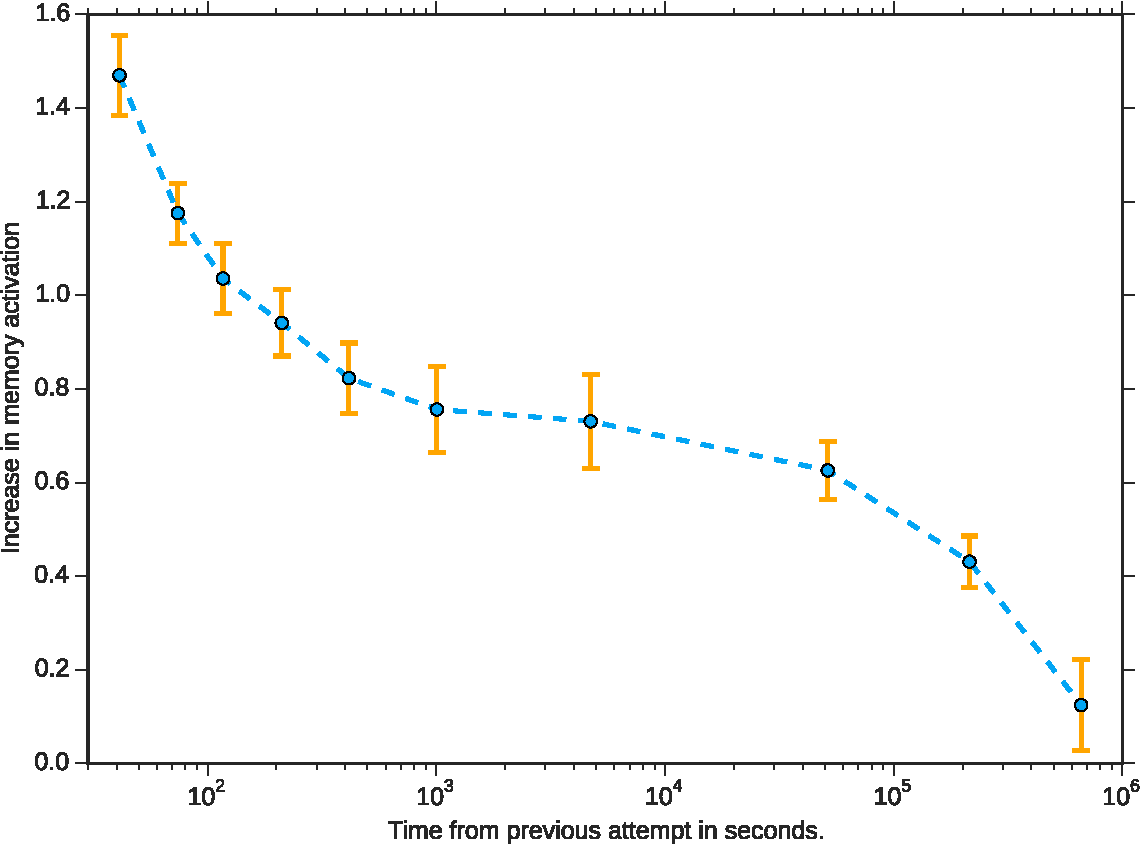
\includegraphics[width=\textwidth]{img/learned-time-effect-function}
  \caption{Time effect function as learned from the data with standard deviations. Each point represents average of 10 independent data sets containing answers of students who used the system continuously at least for one week and answered more than 100 answers.}
  \label{learned-time-effect-function}
\end{figure}

\subsection{Calibration}

Calibration can be used to detect the deviation of model's predictions from the averaged observed frequency of correctness of answers. This is very useful in our case where we need to find out how a model performs with each time effect function over timing distance between concrete practices of individual students. The choice of RMSE isn't very helpful here because it considers all deviations simply as errors in predictions, i.e. it doesn't show whether the model overestimates or underestimates the observed regularity of correct answers. The metric we used in order to calibrate the models is shown in figure~\ref{eq-callibration}.

\begin{equation} \label{eq-callibration}
  \mathit{Correctness} - \mathit{Prediction} = \frac{1}{n} \sum_{i=0}^{n} (y_i - p_i)
\end{equation}

Using a data set of students who practiced geography actively at least for 5 days and answered more than 50 questions, we compared the calibrations for the models that don't account for timing distances between answers. In Figure~\ref{fig:calibration-time-effect-off}, we can see that these models aren't very well calibrated and the analysis suggests that the decay factor introduced in PFA/G doesn't solve this issue. We also analyzed several previously mentioned time effect functions which we used in the PFA/E/T and PFA/G/T models. The Figure~\ref{fig:calibration-time-effect-on} indicates that this method leads to much better calibrated models.

\begin{figure}[htbp]
  \centering
  \begin{subfigure}{.49\textwidth}
    \centering
    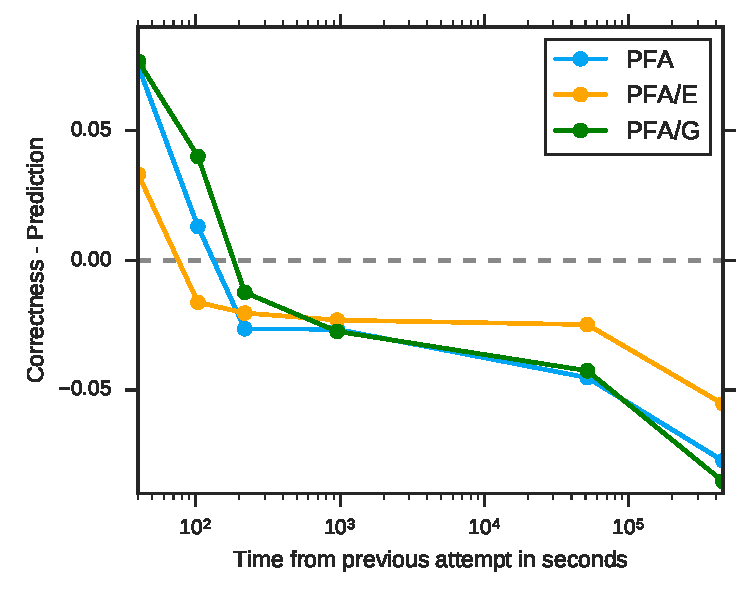
\includegraphics[width=\textwidth]{img/calibration-time-effect-off}
    \caption{}
    \label{fig:calibration-time-effect-off}
  \end{subfigure}
  \begin{subfigure}{.49\textwidth}
    \centering
    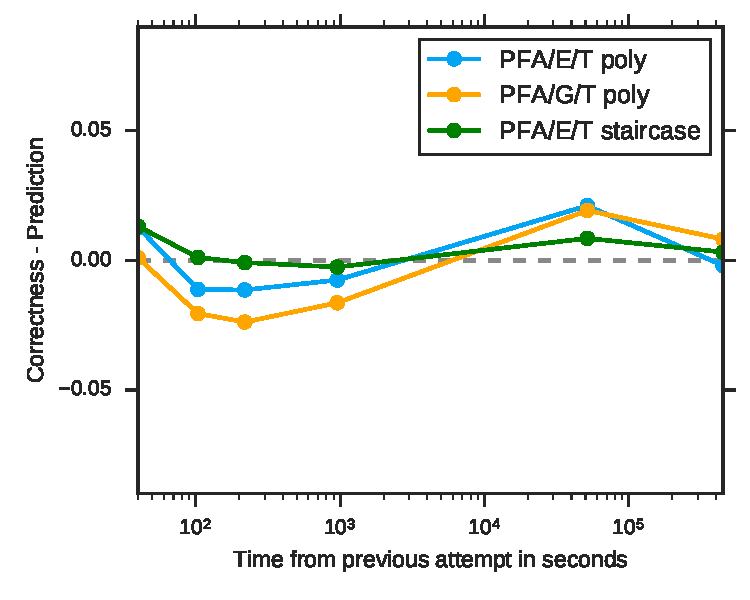
\includegraphics[width=\textwidth]{img/calibration-time-effect-on}
    \caption{}
    \label{fig:calibration-time-effect-on}
  \end{subfigure}
  \label{fig:calibration1}
  \caption{Visualization of calibrations for the plain models (left) and their extended versions with selected time effect functions (right). We learned the parameters of the staircase function from data as was described in chapter~\ref{staircase-function}, the polynomials were estimated using greedy search algorithm.}
\end{figure}

The graphs in Figure~\ref{fig:calibration2} show the comparison of simple time effect functions. The parameters of each model are depicted in Table~\ref{table:calibration2-parameters}.

\begin{table}
  \centering
  \caption{Parameters of calibrated models.}
  \begin{tabular}{ p{2cm}S[table-format=1.3]S[table-format=1.3]
                         S[table-format=1.3]S[table-format=1.3]
                         S[table-format=1.3]S[table-format=1.3] }
   \toprule[\heavyrulewidth]
   & \multicolumn{6}{c}{Time Effect Function} \\
   \cmidrule(r){2-7}
   & \multicolumn{2}{c}{\textbf{log} $= a - c \cdot \log{(t)}$}
   & \multicolumn{2}{c}{\textbf{exp} $= a \cdot e^{-c \sqrt{t}}$}
   & \multicolumn{2}{c}{\textbf{poly} $= a / t^c$} \\
   \cmidrule(r){2-7}
   & \multicolumn{1}{c}{$a$}
   & \multicolumn{1}{c}{$c$}
   & \multicolumn{1}{c}{$a$}
   & \multicolumn{1}{c}{$c$}
   & \multicolumn{1}{c}{$a$}
   & \multicolumn{1}{c}{$c$} \\
   \midrule[\heavyrulewidth]
   \textbf{PFA/E/T} & 1.802 & 0.119 & 1.642 & 0.011 & 2.507 & 0.166 \\
   \textbf{PFA/G/T} & 0.789 & 0.046 & 0.501 & 0.002 & 1.196 & 0.153 \\
   \bottomrule[\heavyrulewidth]
  \end{tabular}
  \label{table:calibration2-parameters}
\end{table}

\begin{figure}[htbp]
  \centering
  \begin{subfigure}{.49\textwidth}
    \centering
    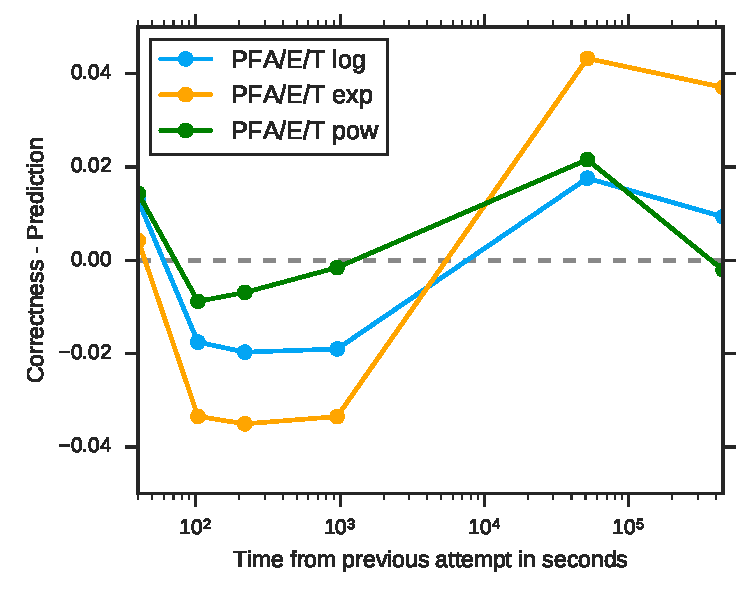
\includegraphics[width=\textwidth]{img/calibration-pfaet}
    \caption{}
    \label{fig:calibration-pfaet}
  \end{subfigure}
  \begin{subfigure}{.49\textwidth}
    \centering
    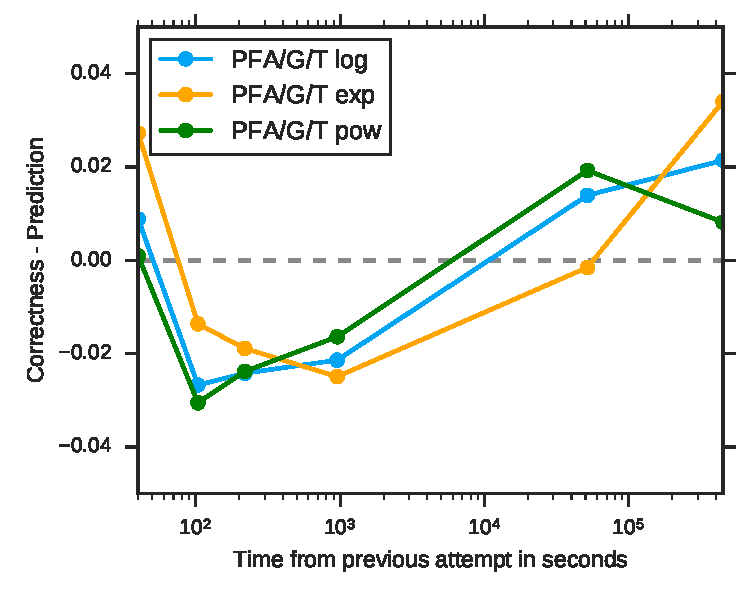
\includegraphics[width=\textwidth]{img/calibration-pfagt}
    \caption{}
    \label{fig:calibration-pfagt}
  \end{subfigure}
  \caption{Visualization of calibrations for the PFA/E/T model (left) and PFA/G/T model (right) with several tested time effect functions.}
  \label{fig:calibration2}
\end{figure}

\section{Evaluation}
\label{evaluation}

We evaluated the models on several different sets of data, including all answers, African and European countries, USA states, Czech rivers, world mountains and also we compared in-school and out-of-school students. Parameters of all models were estimated using either greedy search or gradient descent. For the estimation of prior knowledge we used Elo model where we fitted the parameters $\alpha$ and $\beta$ using grid search algorithm. In Table~\ref{table:results-all-answers} we compare the performance of all evaluated variations of examined models on a data set containing 150 thousand answers.

\begin{table}
  \centering
  \caption{Performance of all variations of models focused on timing information of students' answers. The upper part of the table contains estimated parameters of each model. The lower part consists of scores for each metric. The table is further separated into three sections by a single horizontal line and the best score in each section is marked in bold while the best score overall is underlined.}
  \begin{tabular}{ p{1.8cm} l S[table-format=1.3] S[table-format=1.3]
                   S[table-format=1.3] S[table-format=1.3] S[table-format=1.3] }
   \toprule[\heavyrulewidth]
   \toprule[\heavyrulewidth]
   & \multicolumn{1}{c}{Time effect fun.}
   & \multicolumn{1}{c}{$\gamma$}
   & \multicolumn{1}{c}{$\delta$}
   & \multicolumn{1}{c}{$\xi$}
   & \multicolumn{1}{c}{$a$}
   & \multicolumn{1}{c}{$c$} \\
   \midrule[\heavyrulewidth]
   \textbf{PFA}     & &  1.022 & -0.081 &        &        &        \\
   \textbf{PFA/E}   & &  2.614 & -0.642 &        &        &        \\
   \textbf{PFA/G}   & &  1.798 &  0.091 &  0.425 &        &        \\
   \midrule
   \multirow{4}{4em}{\textbf{PFA/E/T}}
    & $f(t) = a / t^c$                 &  2.004 & -0.713 & &  2.931 &  0.27  \\
    & $f(t) = a - c \log{(t)}$         &  0.119 &  0.119 & &  0.119 &  0.119 \\
    & $f(t) = a \cdot e^{-c \sqrt{t}}$ &  0.119 &  0.119 & &  0.119 &  0.119 \\
    & $f(t) = \mathit{staircase}$      &  1.814 &  0.827 & &        &        \\
   \midrule
   \multirow{3}{3em}{\textbf{PFA/G/T}}
    & $f(t) = a / t^c$                 &  1.610 & -0.02  & &  3.029 &  0.259 \\
    & $f(t) = a - c \log{(t)}$         &  0.119 &  0.119 & &  0.119 &  0.119 \\
    & $f(t) = a \cdot e^{-c \sqrt{t}}$ &  0.119 &  0.119 & &  0.119 &  0.119 \\
   \midrule[\heavyrulewidth]
   \midrule[\heavyrulewidth]
   & \multicolumn{1}{c}{Time effect fun.}
   & \multicolumn{1}{c}{RMSE}
   & \multicolumn{1}{c}{AUC}
   & \multicolumn{1}{c}{LL}
   & \multicolumn{2}{c}{\# of Correct} \\
   \midrule[\heavyrulewidth]
   \textbf{PFA}     & &  0.365 & 0.753 
     & \multicolumn{1}{S[table-format=5]}{-75215}
     & \multicolumn{2}{S[table-format=6]}{118504} \\
   \textbf{PFA/E}   & &  0.346 & 0.8
     & \multicolumn{1}{S[table-format=5]}{-55503}
     & \multicolumn{2}{S[table-format=6]}{120510} \\
   \textbf{PFA/G}   & &  0.35  & 0.782
     & \multicolumn{1}{S[table-format=5]}{-58420}
     & \multicolumn{2}{S[table-format=6]}{120477} \\
   \midrule
   \multirow{4}{4em}{\textbf{PFA/E/T}}
     & $f(t) = a / t^c$                 &  0.341  & 0.806
     & \multicolumn{1}{S[table-format=5]}{-54082}
     & \multicolumn{2}{S[table-format=6]}{121341} \\
     & $f(t) = a - c \log{(t)}$         &  0.231  & 0.982
     & \multicolumn{1}{S[table-format=5]}{-56047}
     & \multicolumn{2}{S[table-format=6]}{156047} \\
     & $f(t) = a \cdot e^{-c \sqrt{t}}$ &  0.231  & 0.982
     & \multicolumn{1}{S[table-format=5]}{-56047}
     & \multicolumn{2}{S[table-format=6]}{156047} \\
     & $f(t) = \mathit{staircase}$      &  0.34   & 0.808
     & \multicolumn{1}{S[table-format=5]}{-54090}
     & \multicolumn{2}{S[table-format=6]}{121238} \\
   \midrule
   \multirow{3}{3em}{\textbf{PFA/G/T}}
     & $f(t) = a / t^c$                 &  0.231  & 0.982
     & \multicolumn{1}{S[table-format=5]}{-56047}
     & \multicolumn{2}{S[table-format=6]}{156047} \\
     & $f(t) = a - c \log{(t)}$         &  0.231  & 0.982
     & \multicolumn{1}{S[table-format=5]}{-56047}
     & \multicolumn{2}{S[table-format=6]}{156047} \\
     & $f(t) = a \cdot e^{-c \sqrt{t}}$ &  0.231  & 0.982
     & \multicolumn{1}{S[table-format=5]}{-56047}
     & \multicolumn{2}{S[table-format=6]}{156047} \\
   \bottomrule[\heavyrulewidth]
   \bottomrule[\heavyrulewidth]
  \end{tabular}
  \label{table:results-all-answers}
\end{table}

\subsection*{European Countries}

\subsection*{African Countries}

\subsection*{USA States}

\subsection*{Czech Rivers}

\subsection*{Mountains}

\subsection*{In-school vs Out-of-school}

\section{Further Analysis}
\label{further-analysis}

\subsection{Confusion Network}

It is natural to mix up places that are geographically very close, have similar names or other reasons. Students typically know the approximate geographic position of Norway but might have confused it's exact position with Finland or Sweden as can be seen in Figure~\ref{confusion-network}. If a students chooses Finland when the highlighted place is actually Norway, it usually doesn't mean that they have no knowledge of the place. In such cases it seems reasonable to take this into account and perhaps even decrease the student's knowledge less significantly.

\begin{figure}[htbp]
  \centering
  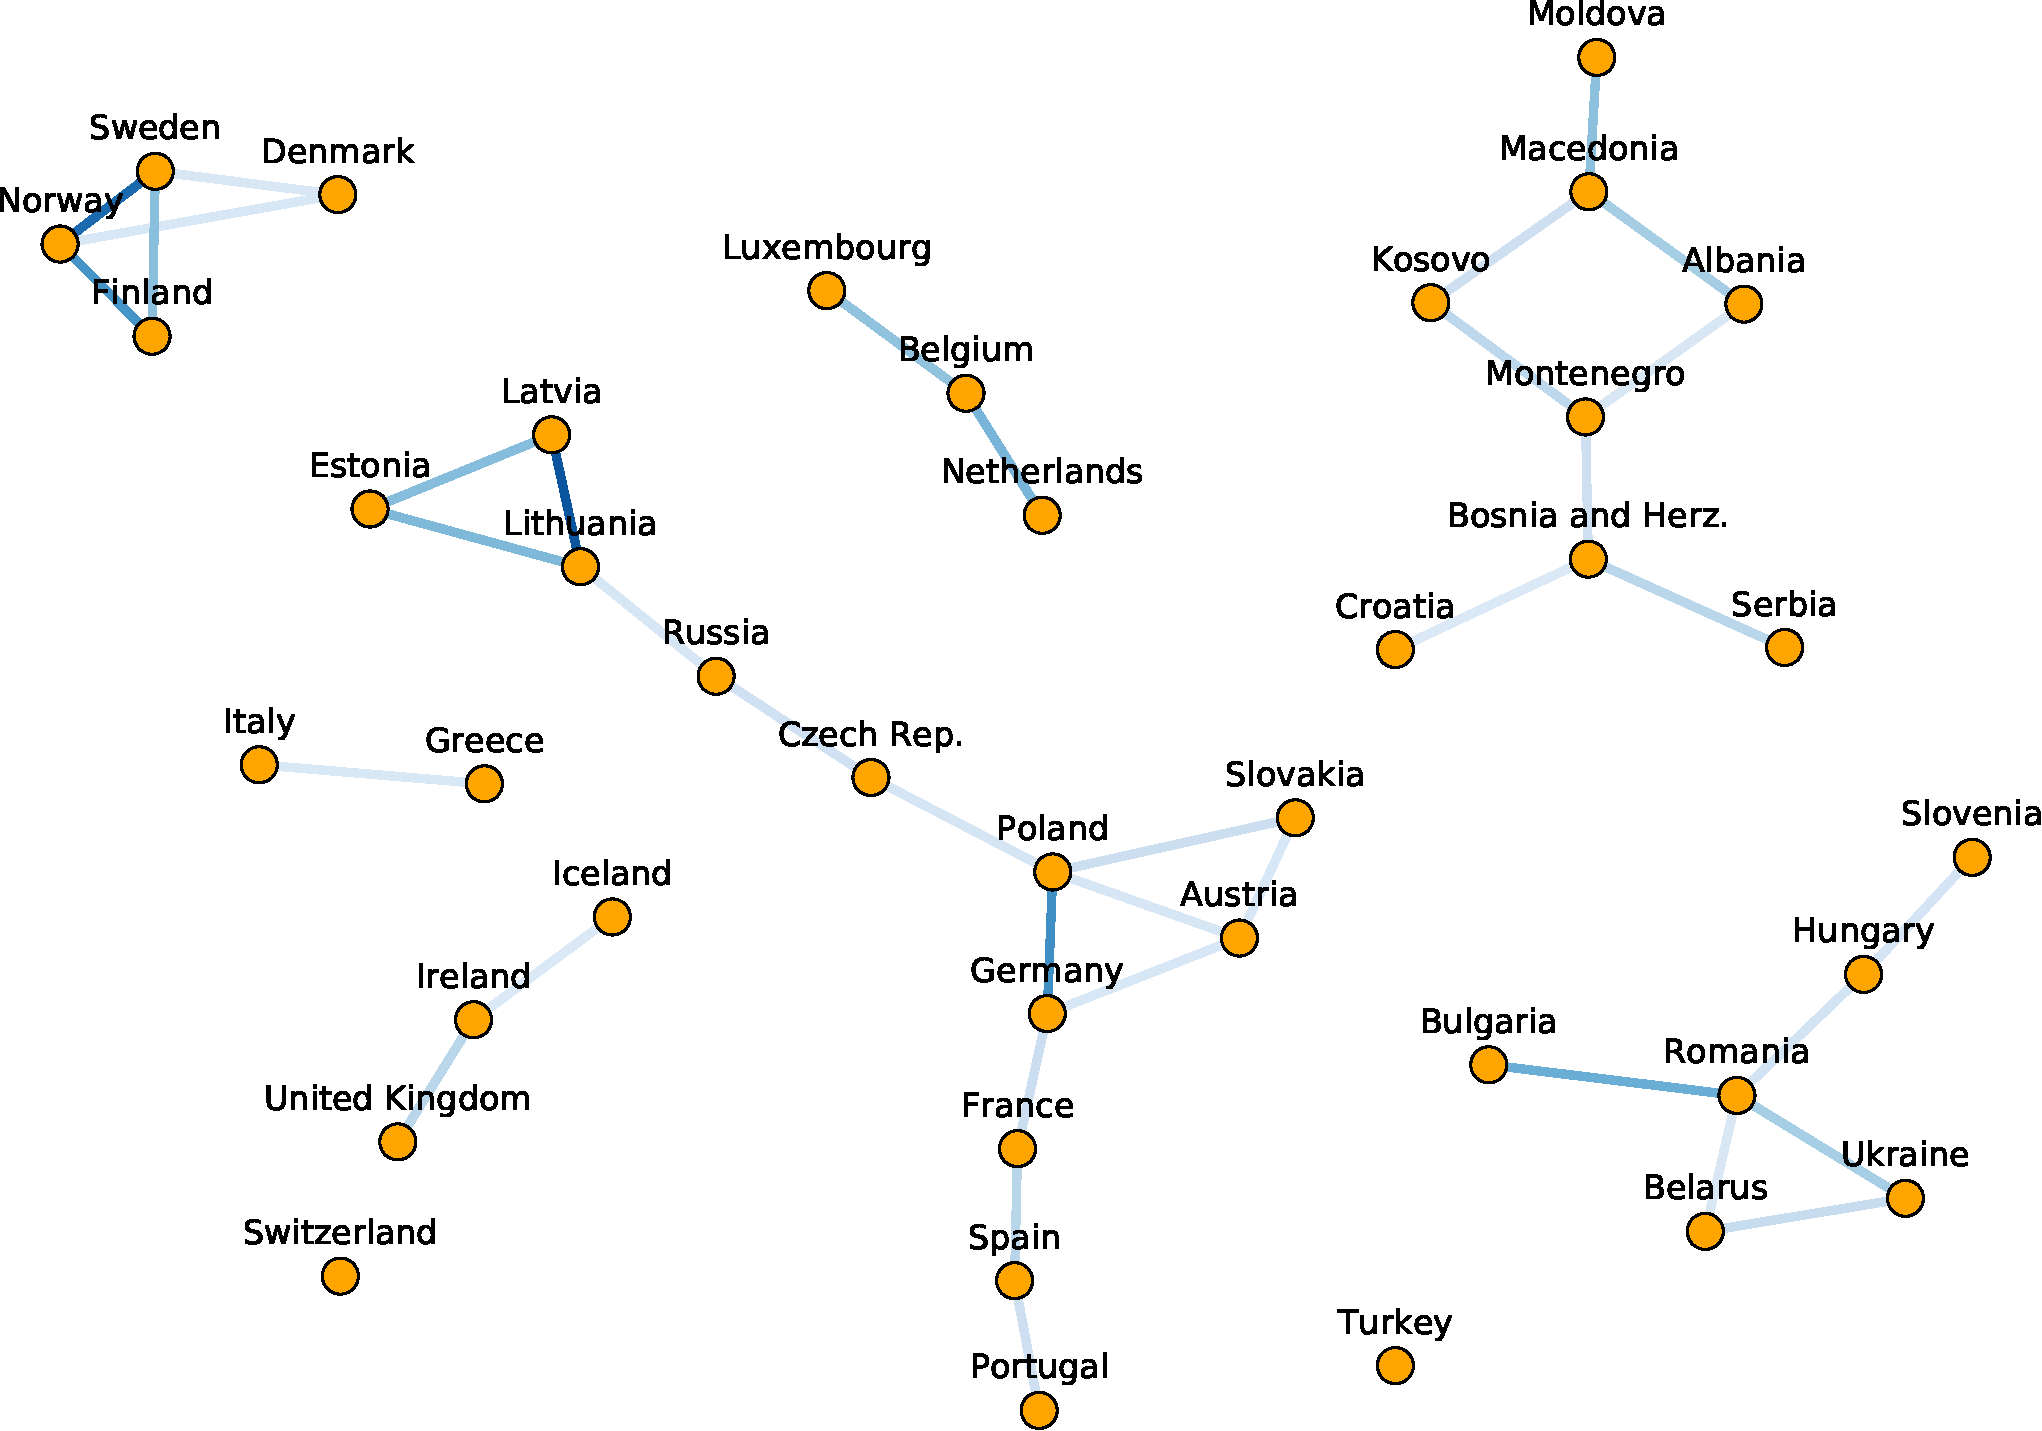
\includegraphics[width=\textwidth]{img/confusion-network}
  \caption{Confusion network of European countries. The edges between countries represent confusion of students. Dark blue edge means that the two connected countries are confused by students quite often while light blue indicates that the countries are still sometimes confused but at least less often.}
  \label{confusion-network}
\end{figure}
